\documentclass{article}
\usepackage[UTF8, scheme = plain]{ctex}
\usepackage{amsmath,amsfonts,amsthm,amssymb,amssymb,amsfonts}
\usepackage{setspace}
\usepackage{fancyhdr}
\usepackage{lastpage}
\usepackage{extramarks}
\usepackage{chngpage}
\usepackage{soul,color}
\usepackage{graphicx,float,wrapfig}
\usepackage{CJKutf8}
\usepackage{graphicx}
\usepackage[noend]{algpseudocode}
\usepackage{algorithmicx,algorithm}
\usepackage{listings}
\usepackage{subfigure}
\newcommand{\Class}{人工智能导论}
%\newcommand{\ClassInstructor}{Jian Li}%

% Homework Specific Information. Change it to your own
\newcommand{\Title}{重力四子棋}
%\newcommand{\DueDate}{Oct 12, 2022}
\newcommand{\StudentName}{周韧平}
\newcommand{\StudentClass}{计 11}
\newcommand{\StudentNumber}{2021010699}

% In case you need to adjust margins:
\topmargin=-0.45in      %
\evensidemargin=0in     %
\oddsidemargin=0in      %
\textwidth=6.5in        %
\textheight=9.0in       %
\headsep=0.25in         %

% Setup the header and footer
\pagestyle{fancy}                                                       %
\lhead{\StudentName}                                                 %
\chead{\Title}  %
\rhead{\firstxmark}                                                     %
\lfoot{\lastxmark}                                                      %
\cfoot{}                                                                %
\rfoot{Page\ \thepage\ of\ \protect\pageref{LastPage}}                          %
\renewcommand\headrulewidth{0.4pt}                                      %
\renewcommand\footrulewidth{0.4pt}                                      %

%%%%%%%%%%%%%%%%%%%%%%%%%%%%%%%%%%%%%%%%%%%%%%%%%%%%%%%%%%%%%
% Some tools
\newcommand{\enterProblemHeader}[1]{\nobreak\extramarks{#1}{#1 continued on next page\ldots}\nobreak%
                                    \nobreak\extramarks{#1 (continued)}{#1 continued on next page\ldots}\nobreak}%
\newcommand{\exitProblemHeader}[1]{\nobreak\extramarks{#1 (continued)}{#1 continued on next page\ldots}\nobreak%
                                   \nobreak\extramarks{#1}{}\nobreak}%

\newcommand{\homeworkProblemName}{}%
\newcounter{homeworkProblemCounter}%
\newenvironment{homeworkProblem}[1][Problem \arabic{homeworkProblemCounter}]%
  {\stepcounter{homeworkProblemCounter}%
   \renewcommand{\homeworkProblemName}{#1}%
   \section*{\homeworkProblemName}%
   \enterProblemHeader{\homeworkProblemName}}%
  {\exitProblemHeader{\homeworkProblemName}}%

\newcommand{\homeworkSectionName}{}%
\newlength{\homeworkSectionLabelLength}{}%
\newenvironment{homeworkSection}[1]%
  {% We put this space here to make sure we're not connected to the above.

   \renewcommand{\homeworkSectionName}{#1}%
   \settowidth{\homeworkSectionLabelLength}{\homeworkSectionName}%
   \addtolength{\homeworkSectionLabelLength}{0.25in}%
   \changetext{}{-\homeworkSectionLabelLength}{}{}{}%
   \subsection*{\homeworkSectionName}%
   \enterProblemHeader{\homeworkProblemName\ [\homeworkSectionName]}}%
  {\enterProblemHeader{\homeworkProblemName}%

   % We put the blank space above in order to make sure this margin
   % change doesn't happen too soon.
   \changetext{}{+\homeworkSectionLabelLength}{}{}{}}%

\newcommand{\Answer}{\ \\\textbf{Answer:} }
\newcommand{\Proof}{\ \\\textbf{Proof:} }
\newcommand{\Acknowledgement}[1]{\ \\{\bf Acknowledgement:} #1}
\newcommand{\D}{\text{ d}}

%%%%%%%%%%%%%%%%%%%%%%%%%%%%%%%%%%%%%%%%%%%%%%%%%%%%%%%%%%%%%
\lstset{ %
	language=C++,                % choose the language of the code
	basicstyle=\fontspec{Consolas},       % the size of the fonts that are used for the code
	%numbers=left,                   % where to put the line-numbers
	numberstyle=\footnotesize,      % the size of the fonts that are used for the line-numbers
	stepnumber=1,                   % the step between two line-numbers. If it is 1 each line will be numbered
	numbersep=5pt,                  % how far the line-numbers are from the code
	backgroundcolor=\color{white},  % choose the background color. You must add \usepackage{color}
	showspaces=false,               % show spaces adding particular underscores
	showstringspaces=false,         % underline spaces within strings
	showtabs=false,                 % show tabs within strings adding particular underscores
	frame=single,           % adds a frame around the code
	tabsize=2,          % sets default tabsize to 2 spaces
	captionpos=b,           % sets the caption-position to bottom
	breaklines=true,        % sets automatic line breaking
	breakatwhitespace=false,    % sets if automatic breaks should only happen at whitespace
	escapeinside={\%*}{*)}          % if you want to add a comment within your code
}

%%%%%%%%%%%%%%%%%%%%%%%%%%%%%%%%%%%%%%%%%%%%%%%%%%%%%%%%%%%%%
% Make title
\title{\textmd{\bf \Class: \Title}}
\author{\textbf{\StudentName}\ \ \StudentClass\ \ \StudentNumber}
%%%%%%%%%%%%%%%%%%%%%%%%%%%%%%%%%%%%%%%%%%%%%%%%%%%%%%%%%%%%%

\begin{document}
\begin{spacing}{1.1}
\maketitle \thispagestyle{empty}
%\cite{}
%%%%%%%%%%%%%%%%%%%%%%%%%%%%%%%%%%%%%%%%%%%%%%%%%%%%%%%%%%%%%
% Begin edit from here
\section{摘要}
\hspace{1.4em} 本次实验中,我尝试用 MCTS 方法设计了重力四子棋游戏智能体,相比传统 MCTS ,我针对游戏规则和评测环境特点进行了一定的优化,包括设计更好的先验策略、加入强剪枝、搜索树节点复用等。同时我还横向比较不同策略设计、公式选择以及参数设置对智能体性能的影响,并提出了可能的解释。最后,针对智能体未来可能的优化方向我提出了一些自己的思考。

\section{基本原理}
	\subsection{蒙特卡洛方法 (MCM)}
	\hspace{1.4em}
	蒙特卡洛方法(Monte Carlo methods)是一类基于概率统计的计算算法,用于通过模拟随机抽样来解决各种复杂问题。该方法得名于蒙特卡洛赌场,因为它使用了随机数(类似于赌博中的抽牌或转轮游戏)来模拟和估计问题的结果。
	蒙特卡洛方法的核心思想是通过大量的随机采样来近似计算问题的解。随着样本数量的增加,近似结果会趋近于真实值,并且可以估计误差范围。这使得蒙特卡洛方法成为处理复杂问题的一种有效工具。 
	\subsection{蒙特卡洛树搜索 (MCTS)}
	\hspace{1.4em} 
	蒙特卡罗搜索树算法是一种基于蒙特卡洛方法的搜索算法,用于解决决策问题,特别是在零和博弈中的最佳决策。它通过在搜索树中模拟游戏的随机走子,并利用蒙特卡洛方法对每个走子位置进行评估,从而选择最优的走子。
	
	蒙特卡罗搜索树算法的基本思想是通过随机模拟游戏的走子,逐步扩展搜索树,并在扩展的节点上使用蒙特卡洛方法进行评估。具体而言,它包含以下几个步骤:
	\begin{itemize}
	\item \textbf{选择}:从根节点开始,根据一定的策略选择子节点进行扩展。通常采用上确界置信区间(Upper Confidence Bound,简称UCB)算法来进行选择,该算法综合考虑了节点的胜率和访问次数。
	
	\item \textbf{拓展}:对选定的子节点进行扩展,生成新的子节点。
	
	\item \textbf{模拟}:从扩展的子节点开始,使用蒙特卡洛方法模拟游戏的随机走子,直到达到终止状态。
	
	\item \textbf{反向传播}:将模拟的结果(例如游戏胜负结果)反向传播回搜索树的节点,更新节点的统计信息,例如访问次数和胜率。
	\end{itemize}

	\begin{figure}[h]
		\centering
		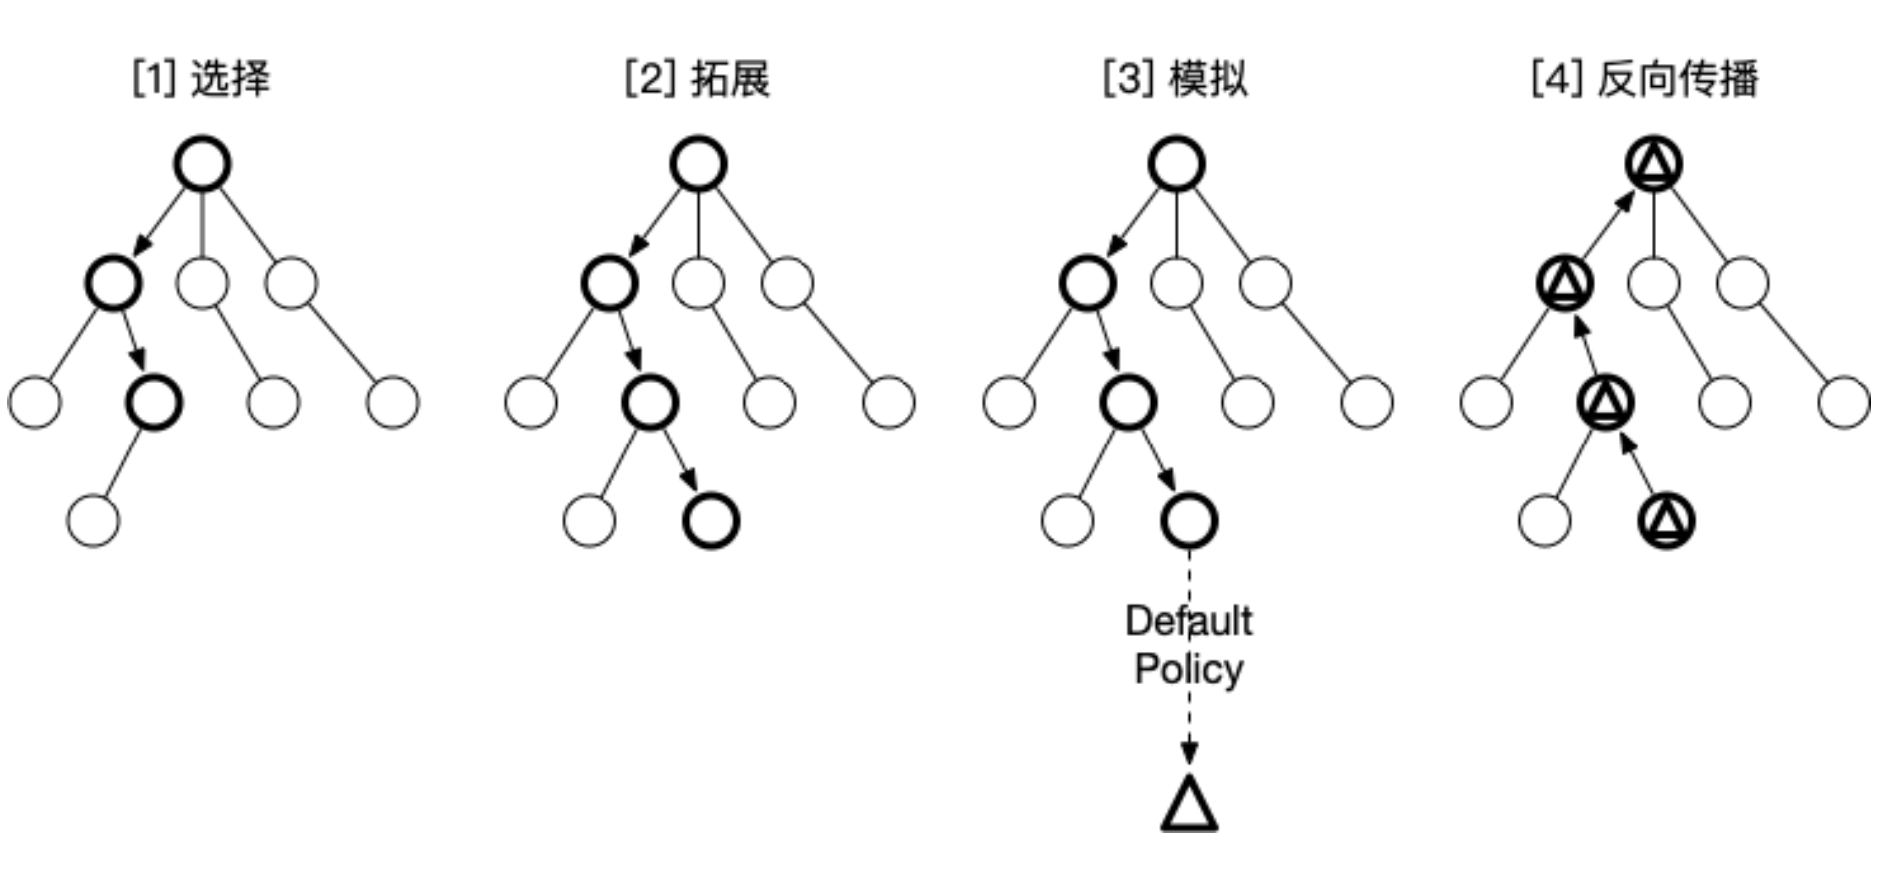
\includegraphics[width=0.8\linewidth]{pic/MCTS.png}
		\caption{MCTS算法示意图}
	\end{figure}
	通过不断重复上述步骤,蒙特卡罗搜索树算法逐渐收敛于最优解,即找到最佳的走子策略。
	
	因此,蒙特卡罗搜索树算法是一种基于蒙特卡洛方法的决策搜索算法,它利用了蒙特卡洛方法的随机模拟和评估能力,在决策问题中寻找最优解。
	
	
\section{具体算法}
	\hspace{1.4em}
	开始阶段,搜索树中只有一个节点,代表当前棋盘局面。搜索树中包含一个用于存储所有节点的节点池(数量上限为 $1.5\times 10^7$ 个结点),其中每个节点记录访问次数、获胜次数。此外,搜索树中还存有两个用于记录棋盘状态的变量,分别记录根节点和当前节点的棋盘状态。
	\subsection{初始化}
	为了避免创建节点池空间可能带来的时间浪费,我选择在一开始就将节点池的空间作为一个全局数组创建出来,并在以后的每次行棋过程中反复使用该片内存
	\subsection{选择}
	\hspace{1.4em}
	在选择阶段,需要从根节点,也就是要做决策的局面 R 出发向下选择出一个最急迫需要被拓展的节点 N,局面 R 是每一次迭代中第一个被检查的节点。
	对于被检查的结点,针对以下三种可能选择最佳节点:
	\begin{itemize}
		\item 如果该节点为叶节点(没有合法孩子),则选择结束,进入扩展
		\item 如果该节点还有没被访问过的节点,则选择该节点。
		\item 如果该节点所有合发子节点都被访问过,则根据 UCB 评分公式:
		$$
		argmax_{v'\in\ childrens\ of\ v} (\frac{Q(v')}{N(v')}+c\sqrt{\frac{ln(N(v))}{N(v')}}) 
		$$
		计算得分最高的节点作为最佳节点。
	\end{itemize}
	\subsection{拓展}
	\hspace{1.4em}
	在拓展阶段,根据拓展策略查找最急切需要被拓展的节点 $N_A$ 作为节点 N 拓展,并返回节点用于模拟,对于拓展策略的设计将在下文详细说明。
	\subsection{模拟}
	\hspace{1.4em}
	对于拓展得到的节点,为了赋予其初始评分,我们从 $N_A$ 开始,让游戏随机进行直到结局,这个结局就是 $N_A$ 的初始得分依据,节点得分定义为 
	$$
	score = \frac{Win\ Counts}{Visit\ Counts}
	$$
	\subsection{反向传播}
	\hspace{1.4em}
	在一次模拟结束后,从节点 $N_A$ 开始,沿着父节点传递这次模拟的结果,并根据更新沿途的节点得分,这里需要注意每个节点定义的得分是“该节点下行棋者的胜率”,因此反传过程中实际上得分是交替变化的。
	 
	\subsection{决策}
	在规定时间内进行了多次迭代后最终得到了一棵规模相当可观的 MCTS 搜索树,最终选择根节点下面的最好节点作为本次决策的最终选择。

\section{算法优化}
	\subsection{移动树根}
	\hspace{1.4em}
	考虑到智能体每两次行棋的状态实际上在 MCTS 搜索树上为祖孙状态的节点,再假设每次 MCTS 搜索树得到结果都可信,则下一次行棋前完全可以利用上一次行棋搜索的结果。这样做一方面相当于增加了迭代的次数,更有可能得到最优的结果;另一方面这样做也更接近人类的思维模式(在下这一步时候就提前思考下面几步的行棋策略,并在之后行棋时参考之前思考的结果)
	此外,这样做的还有一个好处是不用再回收废弃节点,但凡事都是机遇与风险并存,一个首要问题是如此做可能会面临节点池节点用尽的困局,我的方法是当行棋搜索开始前先检查当前节点池已用空间的大小,如果剩余空间低于某个告警值则清空所有节点从头来过。这样做可能会面临盘中因为算力不足导致智能体智力突然下滑的情况,但据我观察只有在棋局开始时节点池的规模扩展迅速,需要反复清空节点池,而在中后期由于树的规模受到相当的限制,几乎不再需要更新节点池,这在一定程度上缓解了该问题可能带来的危害。
	
	\subsection{UCT}
	\hspace{1.4em}
	UCT(Upper Confidence Bounds for Tree) 实际上就是 UCB 和 MCTS 的结合。如上一节中"选择"部分所述,我的算法选择用 $argmax_{v'\in\ childrens\ of\ v} (\frac{Q(v')}{N(v')}+c\sqrt{\frac{ln(N(v))}{N(v')}})$ 作为
	衡量最佳节点的标准。
	除此以外我还进一步参考了其它模型使用的 UCB 公式进行对比实验,如 Muzero 模型中使用的 UCB 公式:
	$$
	a = argmax_a[Q(s,a)+P(a|s)\cdot \frac{\sqrt{1+\sum_b{N(s,b)}}}{1+N(s,a)}(\alpha_1+log(\frac{\sum_b{N(s,b)+\alpha_2+1}}{\alpha_2}))]
	$$
	其中 $Q(s,a)$ 表示该点的得分,本次实验中我用的是胜率。$N(s,a)$ 为执行a操作的次数。$\alpha_1$,$\alpha_2$ 为可以调的超参数。$P(a|s)$ 为一个对状态 s 执行行动 a 的先验概率,在 Muzero 的模型里面需要通过神经网络学习获得,但本次实验中受环境和精力所限我设计的先验策略为:
	\begin{itemize}
		\item \textbf{一击制胜}:如果下完该位置后必胜则一定选择该位置
		\item \textbf{紧急救火}:如果对手下完该位置后必胜则我方一定要选择该位置对其进行封堵
		\item \textbf{随机选择}:如果下一步不存在必胜或者必负策略的话则随机选择合法走子点
	\end{itemize}
	先验策略也为我使用传统UCB公式时的剪枝提供了数学依据,实际上所有的剪枝策略都可以理解为在先验策略中添加的人类智慧。
	
	\subsection{中庸之道}
	\hspace{1.4em}
	一开始我在模拟时使用的是\textbf{随机走子+一击制胜+紧急救火}的策略,这样的策略好处是设计简单且运算速度快,坏处是在模拟一开始缺乏对全局战略的把握,考虑模拟策略在速度和智慧上的平衡,我选择了\textbf{“中庸之道”}作为模拟的策略:考虑到棋盘中央可以向两边发展,应当是“兵家必争之地”,随机模拟时我赋予棋盘中间位置更多的权重,每一个位置的随机权重随距离盘中的位置距离增加而线性递减。
	
	\subsection{三连攻防}
	\hspace{1.4em}
	这是在模拟中添加人类智慧的又一方法。在四子棋、五子棋等游戏中,如果我方出现 n-1 颗棋子相连的情况而两边都为进行封堵,则我方获胜的概率很大。因而当模拟时出现“三联进攻”或者对方制造“三连威胁”时,我方就不应该采取随机走子的策略而应该去创造四连必胜的局面或破坏对方的四连必胜。
	然而在使用该算法时,我面临了性能上比较严重的滑坡,这可能是由于我在局面存储和胜负局面判断上都没有做更多的性能优化,因而导致搜索深度大幅降低,反而出现性能的严重滑坡。
\section{实验结果及分析}
	\hspace{1.4em}
	本次实验中我尝试调整了传统 UCT 公式下调整不同算法中的 \verb|C| 值,搜索时限 \verb|timelimit| 这两个参数进行测试,并对比测试了使用 Muzero 模型提供的 UCB 公式,超参数采用了原论文推荐的值 $\alpha_1 = 19652, \alpha_2 =1.25 $,测试结果如下。
		\begin{table}[h]
		\center
		\begin{tabular}{c|c|c|c}
			\textbf{UCB公式} & \textbf{timelimit} & \textbf{UCB\_C} & \textbf{胜率} \\
			\hline
			UCB1 & 2.0 & 0.707 & \textbf{100}\%\\
			\hline
			UCB1  & 2.0 & 1.0 & 91\%\\
			\hline
			UCB1 & 2.0 & 1.414 & 92\%\\
			\hline
			UCB1 & 2.7 & 0.707 & 96\%\\
			\hline
			UCB1  & 2.7 & 1.0 & 96\%\\
			\hline
			UCB1 & 2.7 & 1.414 & 92\%\\
			\hline
			UCB\_muzero & 2.0 & - & 92\%\\
			\hline
			UCB\_muzero  & 2.7 & - & 96\%\\
		\end{tabular}
		\caption{和12个AI对战测试结果}
	\end{table}


	对打的 AI 为:<<Connect4\_100>><<Connect4\_94>><<Connect4\_92>><<Connect4\_90>><<Connect4\_96>>
	<<Connect4\_98>><<Connect4\_88>><<Connect4\_84>><<Connect4\_80>><<Connect4\_76>>
	<<Connect4\_70>><<Connect4\_64>>

	\textbf{结果分析}:
	\begin{itemize}
	\item 从实验结果来看,搜索时限 \verb|timelimit| 对胜率影响不大,通过对搜索次数的检测也可以发现搜索次数和时限并非线性相关,在搜索时间提升35\%的情况下,搜索次数提升不到10\%。甚至在搜索时限为2.7s时出现了一次较为明显的 collapse 。
	\item  UCB\_1 对智能体表现存在一定的影响,结合实验结果和之前做得大量实验,\verb|C| 取小于1的值表现要好于大于1的值。直观上 \verb|C| 表示的是智能体“尝试新走法”的概率。一般而言,\verb|C| 越大,智能体越激进,实验结果表明,\textbf{该算法在智能体较保守时表现更好}。
	\item \textbf{相比传统 UCB 公式,UCB\_muzero 对智能体表现并没有明显的提升},这可能是因为 UCB\_muzero 中的先验策略不够强导致,毕竟原论文是要用神经网络去学这个公式,不过考虑到 UCB\_muzero 几乎不需要调参,使用上还是要比传统 UCB 公式方便一些。
	\end{itemize}
\section{其它可能的优化方向}
	\subsection{信息储存}
	\hspace{1.4em}
	本次实验中我为了节省空间只在全局存储了两个记录局面状态的变量,相比每个节点都要存储一个状态,我只需要两个变量分别记录根节点状态和当前选择节点状态即可,这节省了大量的空间。进一步,目前我的棋盘通过 int 数组存储,胜负局判断也是通过普通的循环逻辑实现。以后优化的方向可以是通过位运算存储棋盘和判断胜负,如此应该可以提升程序性能,从而增加规定时间内的迭代步数,得到更好的结果。
	\subsection{布置陷阱}
	\hspace{1.4em}
	实验中发现质量较高且在末盘才决出胜负的对局中,往往某几列会出现长时间无人问津的情况,如下图出现的“沟壑纵横”就是经典战例,对于第五列,如果紫色向其中填入棋子,那么黄色方就将获得一击制胜的机会,因而在较长时间内紫色方都不会下该列,黄色方在理想情况下,也不应该下该列,从而给紫色方留下了“陷阱”。总的来说,某一方如果在此处落子,就会为对方创造“一击制胜”的机会,因此这样的列往往要到棋盘全部填满后才被迫填入,这也是很多末盘胜负手的机制。因而,如果能在一开始尽量多的“布设陷阱”,就能获得更高的胜率,这一方法可以添加到模拟中的人类智慧和选择的先验概率中。不过和所有的人类智慧一样,这一方法也需要考虑性能的 trade-of。
	\begin{figure}[h]
		\centering
		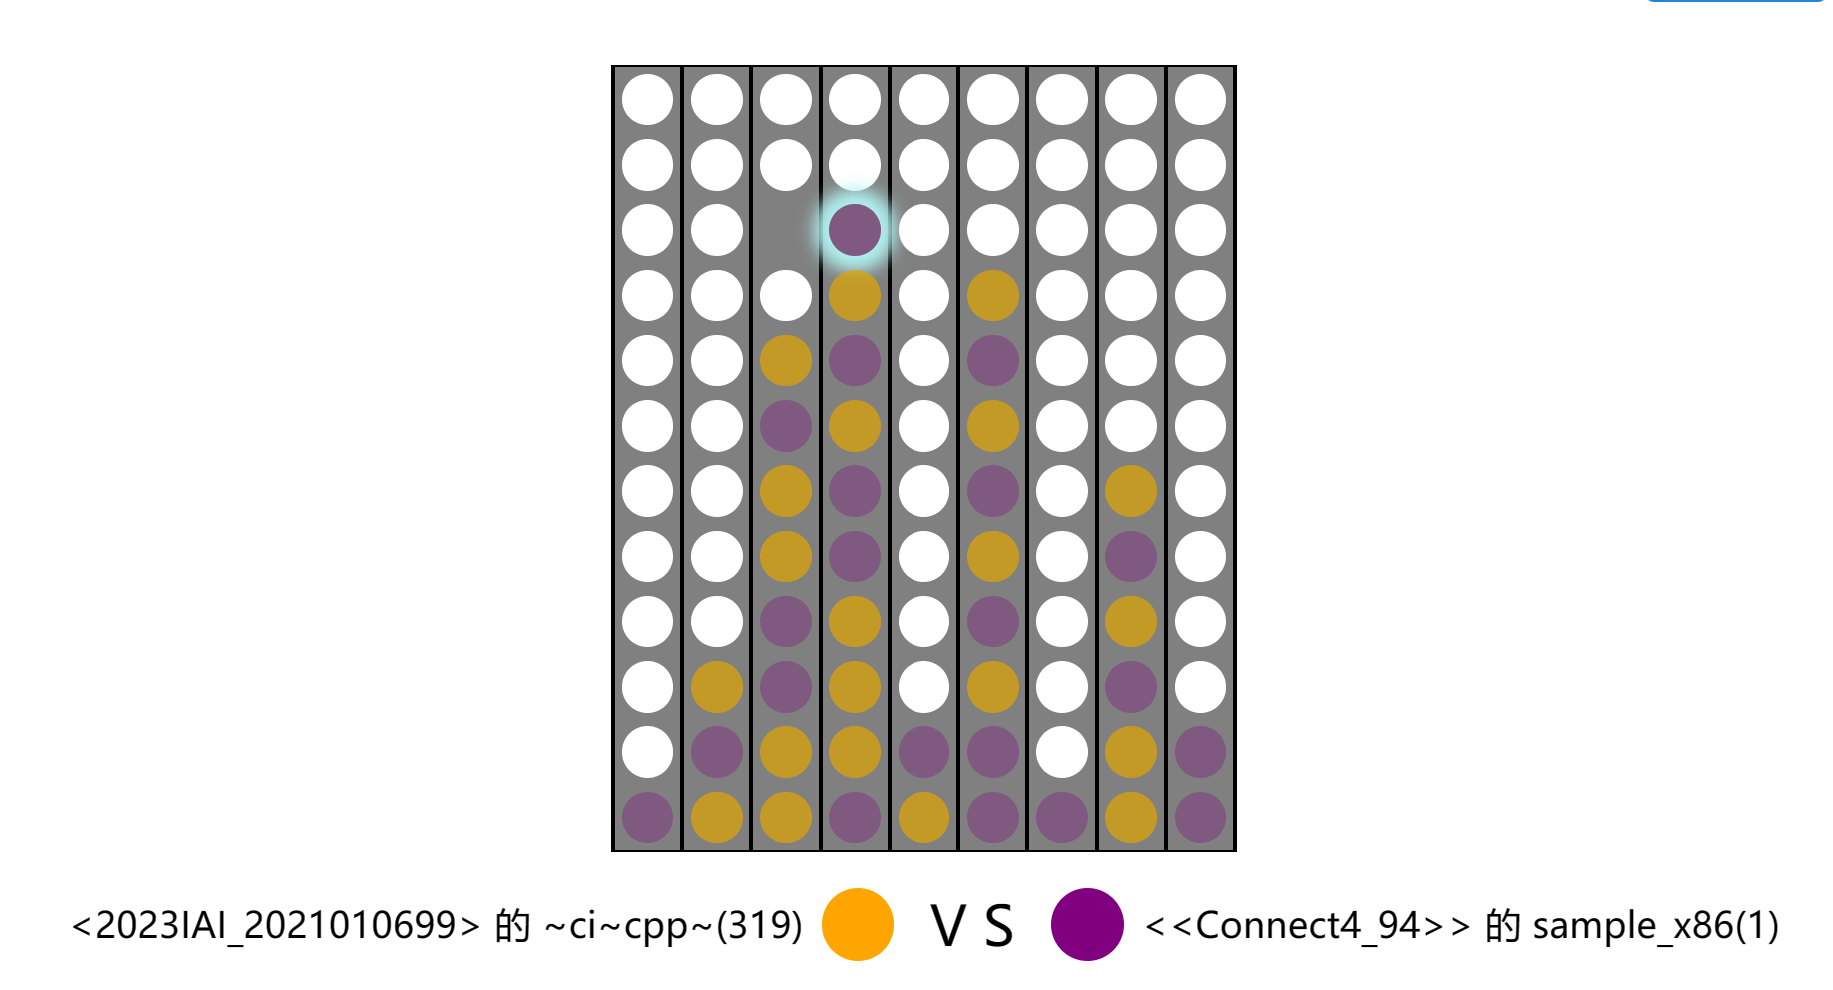
\includegraphics[width=0.8\linewidth]{pic/Trap.png}
		\caption{“陷阱”局面示例}
	\end{figure}
\section{最终结果}
	\hspace{1.4em}
	经过多组实验和尝试,我选择了最稳定的 UCB1 公式+ timelimit=2.7s + UCB\_C=1.0 作为最终上交的智能体版本。该版本在测试中测得胜率在96\%到100\%之间波动,下面是其中一次测试结果展示。
	\begin{figure}[h]
		\centering
		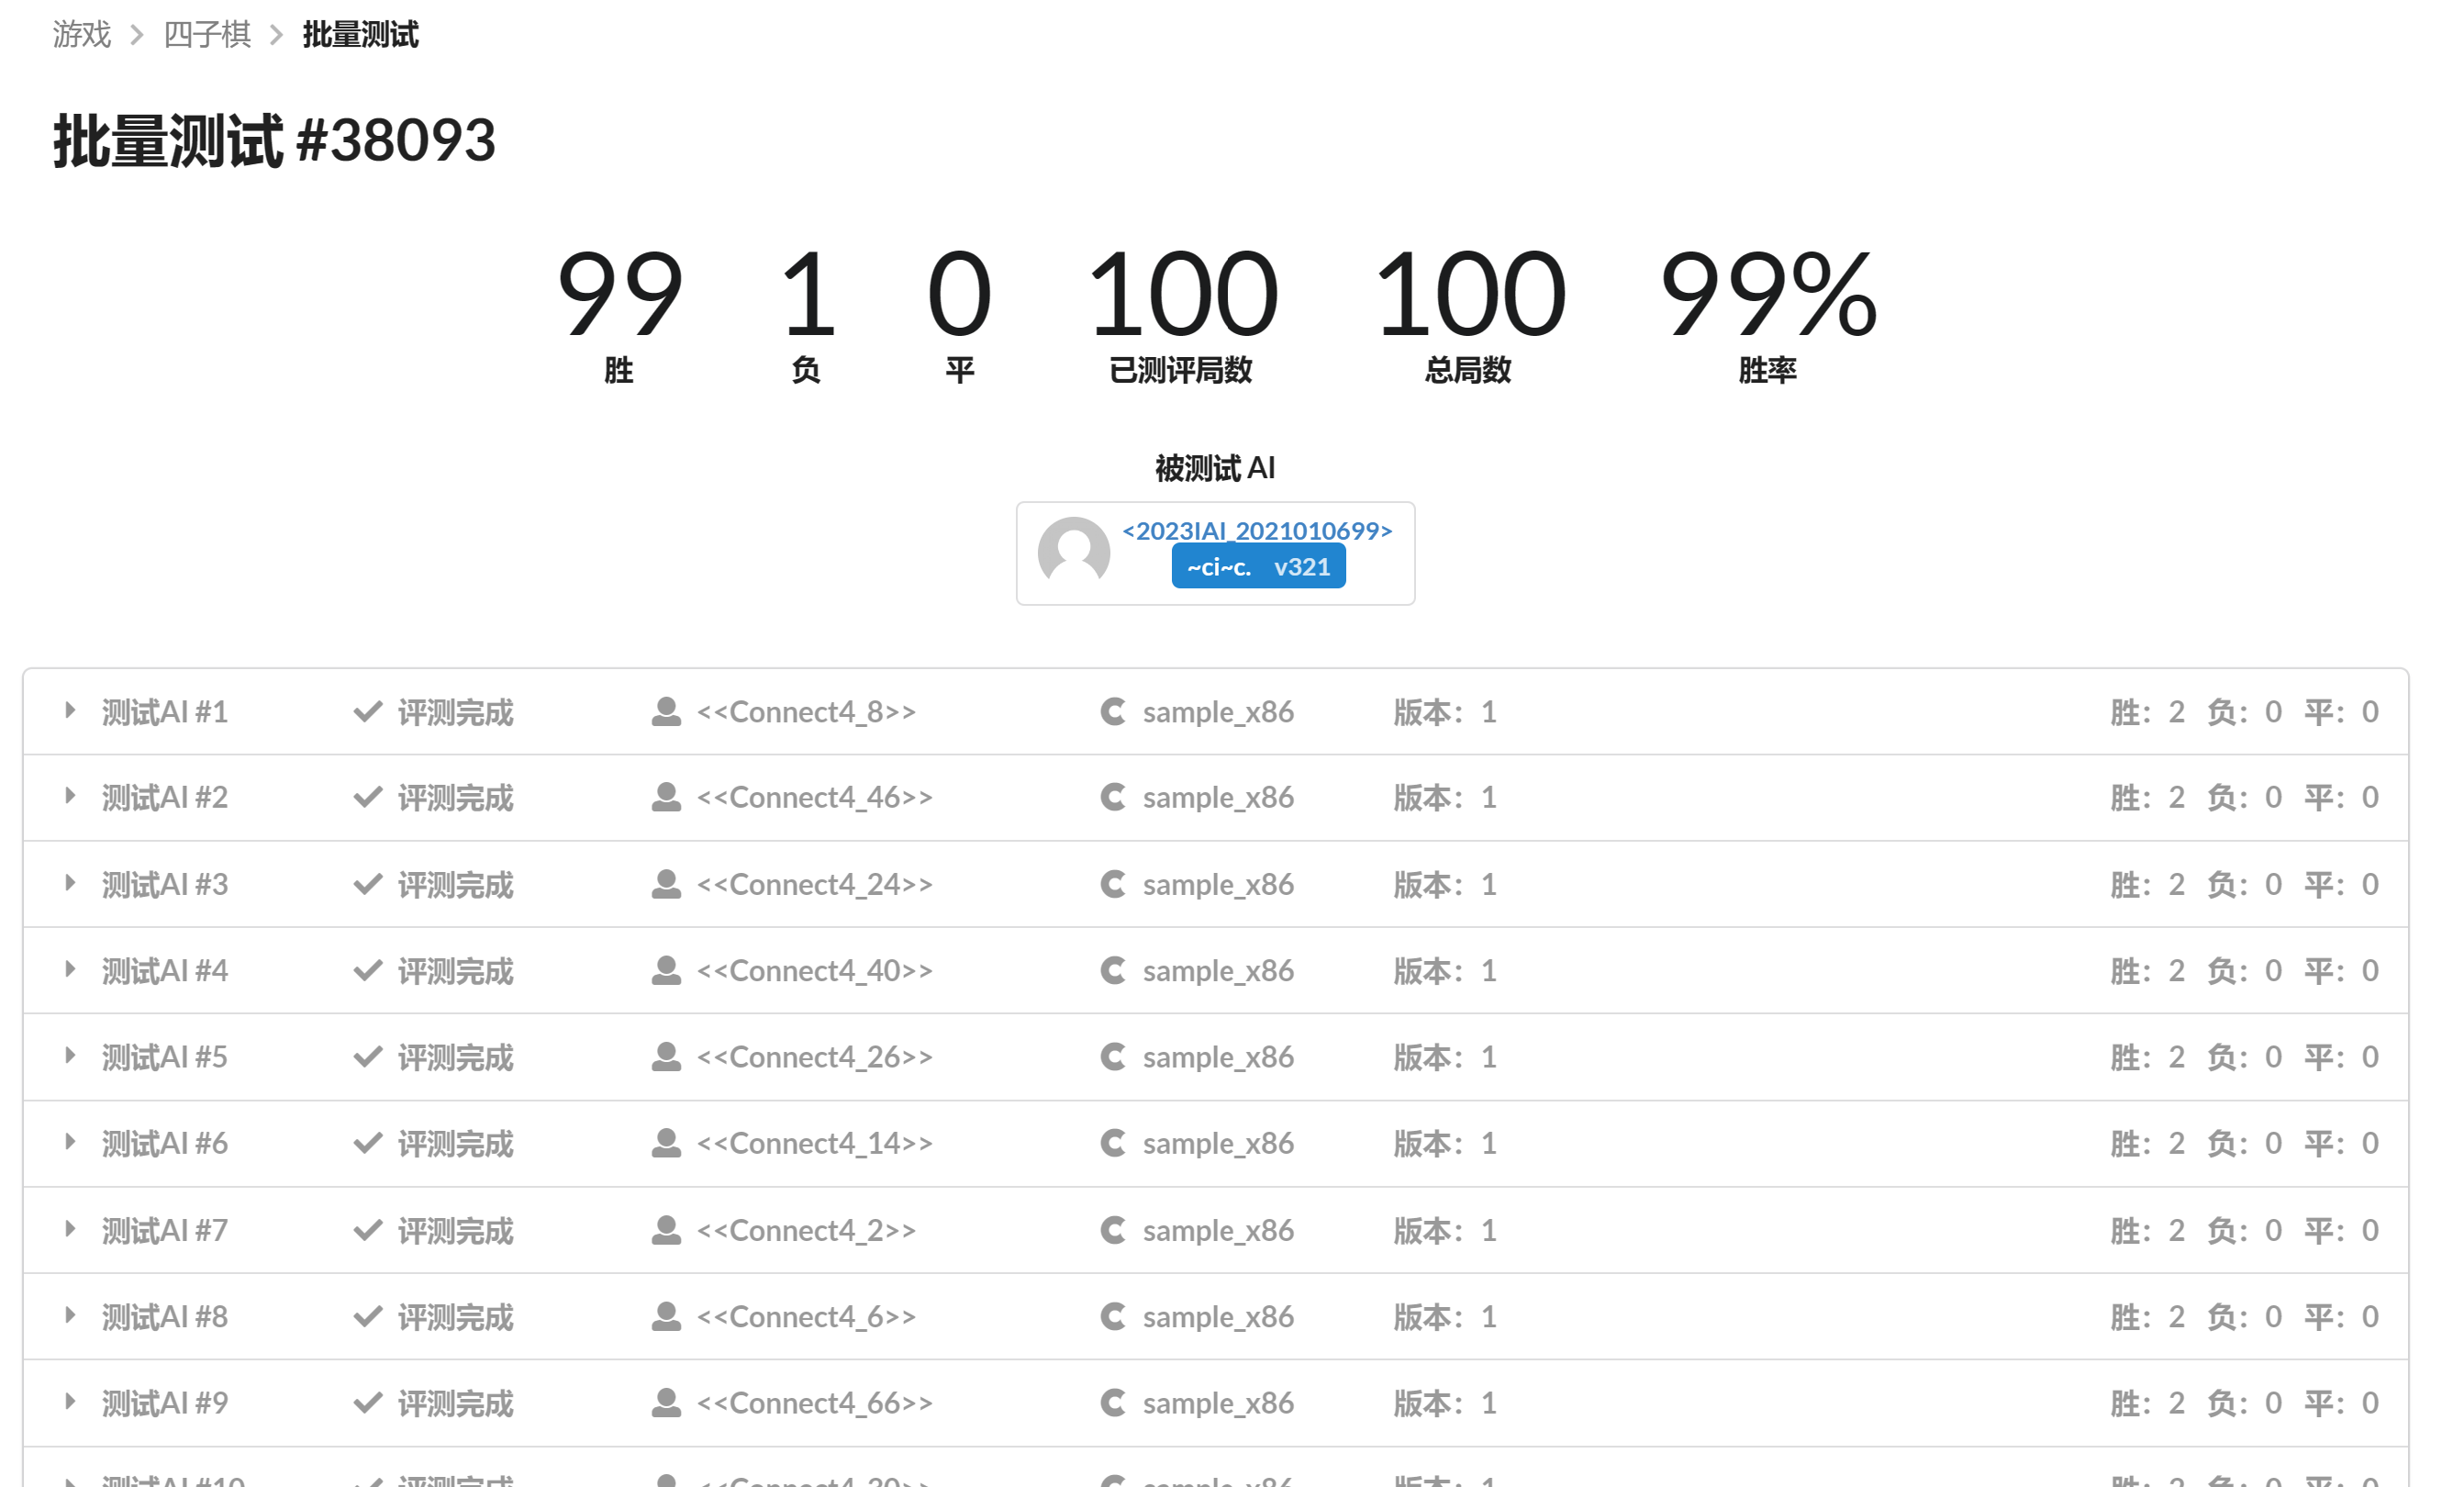
\includegraphics[width=0.8\linewidth]{pic/result.png}
		\caption{测试结果}
	\end{figure}
\section{调试过程}
\hspace{1.4em}	
本次实验代码写的比较不顺,出现了两个比较大的 bug,第一个是节点池大小一开始开的不够导致出现了数组越界访问的问题,线上评测平台并不会对此报错,反而会覆盖数组越界后面指向的那片空间,因此 debug 过程中很难定位到该问题。第二个是在统计每个节点的胜率时我一开始写反了,统计成了负率,导致我的胜率一直在20\%左右徘徊。以上两个bug分别用了我100次 commit 和两三天的时间,commit 次数甚至远超软工,debug过程可谓艰辛。
\section{总结}
\hspace{1.4em}	
本次四子棋实验中,我学习并实现了 MCTS 算法,并在实验和分析中加深了对该算法的理解,同时也练习了寻找问题并优化矛盾的思维方式。
\section{参考资料}
Julian Schrittwieser, Sherjil Ozair, Thomas K Hubert, David Silver, \textit{Planning in Stochastic Environments with a Learned Model Ioannis Antonoglou}
	
% End edit to here
%%%%%%%%%%%%%%%%%%%%%%%%%%%%%%%%%%%%%%%%%%%%%%%%%%%%%%%%%%%%%

\end{spacing}
\end{document}

%%%%%%%%%%%%%%%%%%%%%%%%%%%%%%%%%%%%%%%%%%%%%%%%%%%%%%%%%%%%%
